\chapter{Ejemplos Sencillos}
\label{cap.sencillos}

En este capítulo se aplicarán las ideas del capítulo anterior a ejemplos sencillos. Estudiaremos el operador $A = - \partial ^2 _x$ en el intervalo $[0,L]$ sometido a distintas condiciones de contorno, con este fin se calculará la función-$\zeta$ para luego obtener la energía de vacío. 

En los tres primeros casos se considerará condiciones de contorno Dirichlet, Neumann y periódicas en ambos extremos. Entonces conociendo sus autovalores  se calculara la función-$\zeta$ exactamente. 

En el último ejemplo de este capítulo, se tomará una condición de contorno Dirichlet en un borde y Robin en el otro, de modo de introducir un parámetro externo con dimensiones. Se utilizarán tres técnicas distintas para estudiar la función-$\zeta$: el desarrollo asintótico de los autavalores, una representacion en el plano complejo  y el heat-kernel.

\section{Condiciones de contorno Dirichlet,Neumann y periódicas}
\label{sec.Dirichlet}

En esta sección se estudiarán el espectro y las energía de vacío del operador $A = - \partial ^2 _x$ en el intervalo $[0,L]$ bajo condiciones de contorno Dirichlet,Neumann y periódicas:\\

\subsection*{Condiciones de contorno Dirichlet}


Consideremos primeramente el operador $A$ dado por
\begin{equation}
\begin{aligned}
	A \phi (x) &= - \partial _x ^2 \phi (x) \\[10pt]
    \phi (0) &= \phi(L) = 0 
    \, .
\end{aligned}
\end{equation}
Sus autovalores y autofunciones normalizadas son
\begin{equation}
\begin{aligned}
	\phi _n (x) &= \sqrt{\frac{2}{L}} \sin \left( \frac{n \pi x}{L} \right) \\[10pt]
	\lambda ^2 _n  &= \left( \frac{n \pi }{L} \right) ^2 \, \, \, \, \, n = 1,2,3, \, ...
\end{aligned}
\end{equation}
la  función-$\zeta$ queda determinada por
\begin{equation}
\begin{aligned}
\zeta  (s) &= 
\sum _{n=1} ^{\infty} \left( \frac{\lambda _n }{\mu }  \right) ^{-2s}  \\[10pt]
&= \left(  \frac{\pi}{L \mu} \right) ^{-2s}   \sum _{n=1} ^{\infty} n ^{-2s} = 
\left( \frac{\pi}{L \mu} \right) ^{-2s}  \zeta _R (2s) \, . \\[10pt]
\end{aligned}
\end{equation}
Donde $\zeta _R$ es la función zeta de Riemann definida en la ecuación \ref{rieman-zeta-def}, en el apendice \ref{Apendice.2 se} se demuestra  que $\zeta _R (-1) = - \frac{1}{12}$. 

Por lo tanto resulta que $\zeta (s)$ es regular en $s=-\frac{1}{2}$, siendo la energía de vacío

\begin{equation}\label{eq.energia.dirichlet}
\begin{array}{c}
E _0 = - \frac{\pi}{24 L} \, ,
\end{array}
\end{equation}


Como la energía de vacío crece con $L$, el efecto Casimir implica una fuerza
atractiva entre los extremos del intervalo en el cual está confinado el campo
escalar. Notar que, como la  función-$\zeta$ es regular en $s=-\frac{1}{2}$ el resultado no depende del parámetro de escala $\mu$, tal como se predijo en el capítulo \ref{seq.adim}.\\

\subsection*{Condiciones de contorno Neumann}


Consideremos ahora el operador $A$ dado por.

\begin{equation}
\begin{aligned}
	A \phi (x) &= - \partial _x ^2 \phi (x) \\[10pt]
    \phi ' (0) &= \phi ' (L) = 0 \, ,
\end{aligned}
\end{equation}
cuyos autovalores y autofunciones están dados por
\begin{equation}
\begin{aligned}
	\phi _0 (x) &= \sqrt{ \frac{1}{L} } \\[5pt]
	\phi _n (x)  &= \sqrt{\frac{2}{L}} \cos \left( \frac{n \pi x}{L} \right) 
	\, \, \, \, \, \, n \neq 0\\[5pt]
	\lambda ^2 _n  &= \left( \frac{n \pi }{L} \right) ^2 
	\, \, \, \, \, \,
	n = 0,1,2,3, \dots
	\\[5pt]
\end{aligned}
\end{equation}


Como el cálculo de la {\it función-$\zeta$} se realiza excluyendo los modos cero, la
energía de vacıío coincide con la calculada anteriormente para condiciones
de contorno Dirichlet.\\


\subsection*{Condiciones de contorno periódicas}


Estudiemos ahora el mismo operador bajo condiciones de contorno periódicas
\begin{equation}
\begin{array}{c}
	A \phi (x) = - \partial _x ^2 \phi (x) \\[5pt]
    \phi (0) = \phi (L)  \\[5pt]
    \phi ' (0) = \phi ' (L) \, ,
\end{array}
\end{equation}
Este problema representa una partícula escalar confinada en un anillo $S ^1$ .
Los autovalores y autofunciones están dados por
\begin{align}
	\phi _{0} &= \sqrt{\frac{1}{L}} \\[5pt]
	\phi _{n} (x) &= \sqrt{\frac{2}{L}} \cos \left( \frac{2 n \pi x}{L} \right),
	\, \, \,  \psi _n (x) =\sqrt{\frac{2}{L}} \sin \left( \frac{n \pi x}{L} \right) 
	\, \, \, \, \, \, \, \, \, n \neq 0
	\\[5pt]
	\lambda ^2 _n  &= \left( \frac{2 n \pi }{L} \right) ^2 
	\, \, \, \, \, \, \, \, \,
	 n = 0,1,2,3, \dots
\end{align}
La función-$\zeta$ resulta
\begin{equation}
\begin{aligned}
\zeta  (s) &= 
2 \sum _{n=1} ^{\infty} \left( \frac{\lambda _n}{\mu ^2} \right)^{-s} \\[5pt]
&=  2 \left( \frac{2 \pi}{L} \right) ^{-2s} \mu ^{2s} \sum _{n=1} ^{\infty} n ^{-2s} =  
2 \mu ^{2s} \left( \frac{2 \pi}{L} \right) ^{-2s} \zeta _R (2s)
\, ,
\end{aligned}
\end{equation}
que al igual que en los casos anteriores es regular en $s=- \frac{1}{2}$. Obtenemos
entonces la energía de vacío
\begin{equation}
E _0 = - \frac{\pi}{6 L}
\end{equation}
Nuevamente, la energía crece con L, lo que señala una fuerza que tiende a
reducir el tamaño del anillo.

\section{Condiciones de Contorno Mixtas}


Introducimos ahora un parámetro $S$ con dimensiones, a partir de condiciones de contorno Robin en uno de los extremos del intervalo,
\begin{equation}
\begin{aligned}
    A \phi (x) &= - \partial ^2 _x \ \phi (x)  \\[5pt]
    \phi (0) &= 0 \\[5pt]
    \phi ' (L) + S \phi (L) &= 0 \, .
\end{aligned}
\end{equation}
Las autofunciones con autovalor no nulo son
\begin{equation}
\phi _n (x) = 
B _n \sin ( \lambda _n x ) \, .
\end{equation}
Donde $B_n$ es una constante de normalización. El espectro de autovalores no nulos $\lambda _n \neq 0 $ está dado por
\begin{align}
    \lambda _n   \cos( \lambda _n L) +  S \sin( \lambda _n L) &= 0
    \, . \label{autovalores2} 
\end{align}
Una vez obtenidos los autovalores, calcularemos la {\it función-$\zeta$}
\begin{equation}
    \zeta (s) =  \sum_{n = 1} ^{ \infty } \left( \frac{\lambda _n}{\mu } \right) ^ {-2 s} \, ,
    \tag{\ref{eq.casimir.mu}}
\end{equation}
la dificultad está en que las ecuación (\ref{autovalores2}) no provee una solución explícita para $\lambda _n$. Para estudiar la función-$\zeta$ utilizaremos tres técnicas: la primera de ellas consiste en obtener un desarrollo asintótico de los autovalores, la segunda utiliza una representación integral en el plano complejo de la función-$\zeta$, y la tercera se basa en la relación con el {\it heat-kernel}. 

\subsection{Desarrollo Asintótico de los autovalores}{\label{seq.asin}}

Primeramente, definimos variables adimensionales $\rho _n = \lambda _n L $ y $\theta = S L $, de modo que la ecuación (\ref{autovalores2}) se puede expresar de la forma
\begin{equation}
    \tan (\rho _n) + \frac{\rho _n}{\theta} = 0
    \, .
    \label{eq.asintota}
\end{equation}
En la figura \ref{fig:Dibujo1} están graficados los dos terminos de \ref{eq.asintota}. Puede verse que los autovalores $\rho _n$ tienden a las asíntotas verticales de $ \tan ( \rho ) $ a medida que $\rho _n$ crece. Por consiguiente, escribimos para los autovalores $\rho _n$ 
\begin{align}
    & \rho _n = n \pi + \frac{\pi}{2} + \epsilon _n 
\label{eq.mu}    
\\[5pt]
\nonumber
    & \lim \limits_{ n \rightarrow \infty} \epsilon _n = 0
\, ,
\end{align}
\begin{figure}
    \centering
    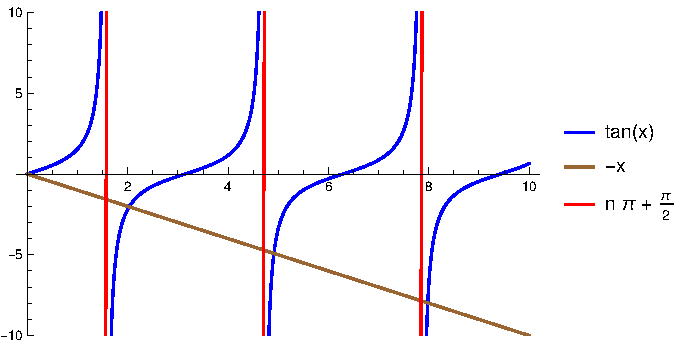
\includegraphics[scale=0.6]{Dibujo.pdf}
    \caption{En este ejemplo, se puede ver que la intersección entre $ \tan(x)$ y $-x$ tiende a las asíntotas verticales de $\tan (x) $, el mismo comportamiento se aprecia para cualquier recta de la forma $- a x$.}
    \label{fig:Dibujo1}
\end{figure}
Utilizando esta expresión de $\rho _n$ en la ecuación \eqref{autovalores2} se obetiene una ecuación para $\epsilon _n$
\begin{equation}
\begin{aligned}
    \sin \left( n \pi + \frac{\pi}{2} + \epsilon _n \right) = -
    \frac{n \pi + \frac{\pi}{2} + \epsilon _n}{\theta} \cos \left( n \pi + \frac{\pi}{2} + \epsilon _n\right)
    \, ,
\end{aligned}
\end{equation}
para lograr obtener una expresión de $\epsilon _n$ se desarrolla la ecuación anterior alrededor de $\epsilon  _n \sim 0$, obteniendo 
\begin{equation}
    1 = 
    \sum _{p=0} ^{\infty} (-1) ^p     \left[
   	\left( \frac{1}{\theta (2p+1)!  } + \frac{1}{(2p+2)!} \right) \epsilon _n ^{2p+2 } +
  	\frac{n \pi + \frac{\pi}{2}}{\theta (2p+1)! }   \epsilon _n ^{2p+1} 			\right]
  	\, .
\label{igualdad epsilon}
\end{equation}
A partir de esta expresión, como solamente existen potencias enteras de $\epsilon$, se propone un desarrollo de  $\epsilon _n$ de la forma
\begin{equation}
\label{eq.epsilon}
    \epsilon _n = 
    \frac{\epsilon ^{(1)}}{n}  + 
    \frac{\epsilon ^{(2)}}{n ^2}  + 
    \frac{\epsilon ^{(3)}}{n ^3}  + \dotsb
\end{equation}
Reemplazando esta propuesta de desarrollo en la ecuación \eqref{igualdad epsilon}, y resolviendo término a término se obtiene para $\epsilon _n $
\begin{equation}
    \epsilon _n = \frac{\theta}{n \pi} 
     - \frac{ \theta}{2 \pi n ^2 } + O \left( n ^{-3}\right) 
     \, .
\label{epsilons}
\end{equation}
Utilizando estos resultados en la definición de función-$\zeta$ dada \eqref{def.adim} se obtiene
\begin{align}
\nonumber
    \zeta  (s) &=  
    \sum _{n=1} ^{\infty} 
    \left( \frac{\lambda _n }{\mu } 
    	\right) ^ {- 2s}  \\
&=
\label{eq.abajo.chi}
    \mu ^{2s} \sum _{n=1} ^{\infty} 
    \left(
	\frac{n \pi}{L } + 
    \frac{\pi}{2 L } +
    \frac{S}{n \pi } -
    \frac{S}{2 \pi n ^2   } +
    O \left(  n^{-3} \right) 
    \right) ^{-2 s}  \\[5pt]    
&= 
\nonumber
	\left( \frac{L \mu }{\pi} \right) ^{2s}    
    \sum _{n=1} ^{\infty} 
    n ^{- 2 s} 
    \left(
    1 +     
    \underbrace{
        \frac{1}{2 n} + 
        \frac{L S}{n^2 \pi ^2} -
        \frac{L S}{2 n ^3 \pi ^2} } 
        _{ \chi _n} +
        O \left(n ^{-4} \right)  
    \right ) ^{-2 s}
    \, .
\end{align}
De manera consistente con los términos  $ O (n ^{-4})$ que no hemos calculado, desarrollamos el binomio para pequeños valores de $\chi _n$ hasta el orden cúbico,
\begin{align}
\label{eq.auxiliar2}
\zeta  (s) &= 
\left( \frac{L \mu }{\pi} \right) ^{2 s}
\sum _{n=1} ^{\infty}
  n  ^{-2 s} \times \\[5pt]
& \times   \ \Bigg(
	1 - 
	2 s \chi _n +  s(2s+1) \frac{\chi _n ^2}{2} - 
	\frac{2}{3} s(2s+1)(s+1) \chi _n ^3  + O \left( n ^{-4} \right) \Bigg)
	\, .
	\nonumber
\end{align}
Dado que los términos $\chi _n ^p$ son polinomios en $\frac{1}{n}$, $\zeta(s)$ puede entonces escribirse en términos de la función zeta de Riemann $\zeta _R (s)$
\begin{align}
    \zeta  (s) &= \left( \frac{L \mu }{\pi} \right) ^{2s} \times 
\\[5pt]
\nonumber
&
\times
	 \Bigg(
		\zeta _R ( 2 s ) -
		s \zeta _R ( 2s+1 ) +
		 s \left( \frac{1}{4} + \frac{s}{2} - \frac{2 L  S}{\pi ^2} \right) \zeta _R (2s +2 ) - \\[5pt]
\nonumber
		 &  \left(  
					\frac{s(s+1) ( \pi ^2 + 2 \pi ^2 s - 24 L S)}{12 \pi ^2 }
		 			\right) \zeta _R (2s+3)
		+ \sum _{n=1} ^{\infty} n ^{-2s} O ( n ^{-4})
		\Bigg)
		\, .
\end{align} 
Los siguientes términos de $\zeta (s)$ son de la forma $\sum _{n=1} ^{\infty} n ^{-2s} O ( n ^{-p})$, los cuales cumplen la propiedad
\begin{align}
	\sum _{n=1} ^{\infty} n ^{-2s} O ( n ^{-p}) 
	\propto
	\zeta _R (2s+p)
	\, ,
\end{align}
donde $\zeta _R (2s+p)$ es una función meroforma con polo simple en $s = \frac{1}{2} - \frac{p}{2}$,
por lo tanto los polos de $\zeta (s)$ quedan caracterizados por los polos simples de las funciones  $\zeta _R (2s+p)$. De esta manera se muestra que $\zeta (s)$ posee polos simples en los semi-enteros negativos, de acuerdo con el el resultado \eqref{eq.ceros.zeta}. El desarrollo hasta orden $O(n^{-3})$ que hemos calculado para los autovalores permite obtener los residuos correspondientes a los siguientes polos.
\begin{equation}
\begin{aligned}
\left(1- \frac{1}{2} \right) \zeta  (s)| _{s=\frac{1}{2}} &= 
\frac{L \mu }{2 \pi } \\[5pt]
s \zeta  (s) |_{s=0} &= \ 0 \\[5pt]
\left( s + \frac{1}{2} \right)\zeta  (s) | _{s=-\frac{1}{2}} &= \frac{S}{2 \pi \mu } \\[5pt]
(s+1) \zeta (s) |_{s=-1} &=  0
\, ,
\\[5pt]
\end{aligned}
\label{eq.polos.asin}
\end{equation}



\subsection{Representación integral de la función $\zeta$}
{\label{sec.complejo}}

En la sección \ref{seq.asin} se calculó un desarrollo de los autovalores y luego se
los utilizó en la definición (\ref{def.adim}) para obtener
la estructura de polos de la función $\zeta$. En este capítulo estudiaremos la
estructura analítica de $\zeta (s)$ de una manera alternativa, que será de utilidad
más adelante.

Supongamos que los autovalores $\lambda ^2 _n$ están definidos por una expresión de
la forma $f ( \lambda ^2 _ n ) = 0$ y que $\lambda ^2 _n$  son ceros simples de la función analítica $f (z)$.
En ese caso, la función $( \log f (z))'$ tiene polos simples en $\lambda ^2 _n$ con residuo 1.
Utilizando el teorema de los residuos, la función $\zeta (s)$ se puede representar
como una integral en el plano complejo cuyo camino de integración $C$
encierra los ceros de $f (z)$ (véase la figura \ref{fig:contorno}),
\begin{equation}
\begin{aligned}
   \zeta  (s) &=  \sum _{n=1} ^{\infty} \left( \frac{\lambda _n}{\mu} \right) ^{-2s} 
   =  
   \frac{1}{2 \pi i} \int _{C} \frac{f'(z)}{f(z)} \left( \frac{z}{\mu} \right) ^{-2s} dz 
\end{aligned}
\label{asd}
\end{equation}
En el problema que estamos considerando $f(z) = z \cos Lz + S \sin Lz$ (ver (\ref{autovalores2})). Reemplazando en la representación integral obtenemos
\begin{equation}
	\zeta  (s) = 
    \frac{\mu ^{2s}}{2 \pi i} \int _{C}
    \frac{ \cos (L z) \left(L + \frac{1}{S} \right) - \sin(L z) \frac{z L}{S}
    }
    { \cos(L z) \frac{z}{S} + \sin(L z)
    }
     z  ^{-2 s} dz  \, .
\end{equation}
\begin{figure*}[t!]
    \centering
    \begin{subfigure}[t]{0.3\textwidth}
        \centering
        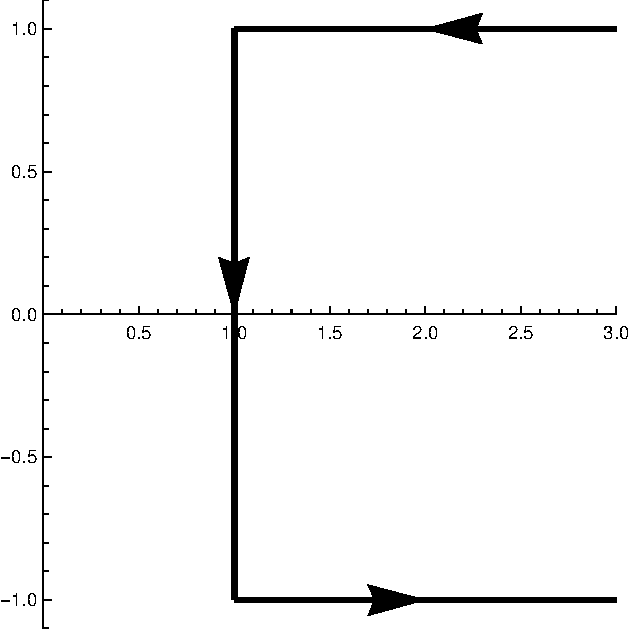
\includegraphics[height=1.2in]{Camino.pdf}
        \caption{}
        \label{fig.izquierda}
    \end{subfigure}%
    ~ 
    \begin{subfigure}[t]{0.3\textwidth}
        \centering
        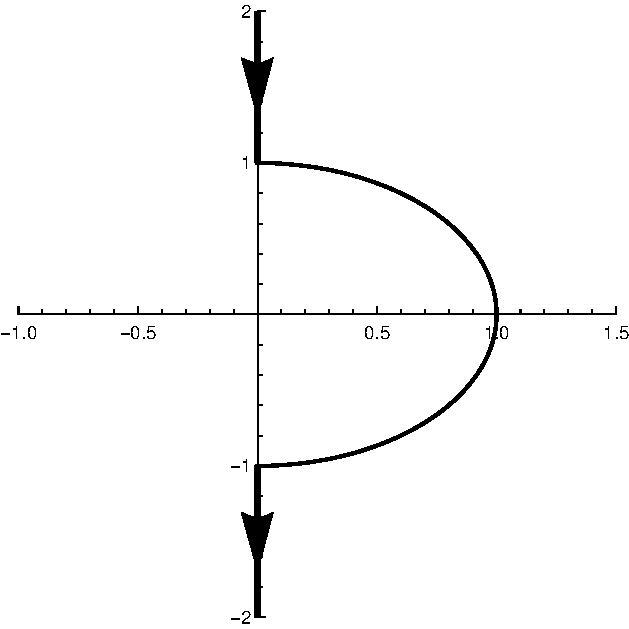
\includegraphics[height=1.2in]{Camino2.pdf}
        \caption{}
        \label{fig.derecha}
    \end{subfigure}
    ~
    \begin{subfigure}[t]{0.3\textwidth}
        \centering
        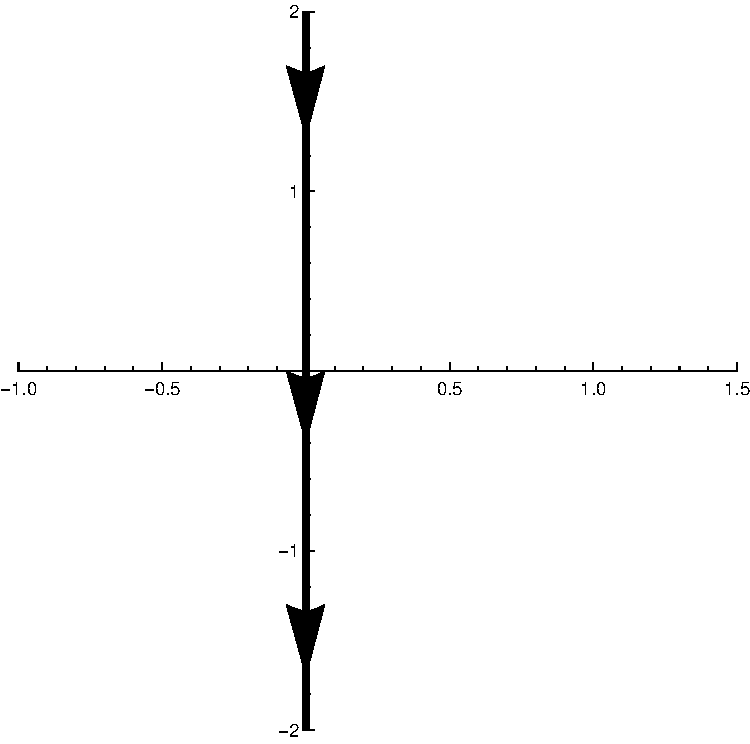
\includegraphics[height=1.2in]{Camino3.pdf}
        \caption{}
        \label{fig.derecha.derecha}
    \end{subfigure}
    \caption{Estos caminos son los tenidos en cuenta para representar a la {\it función-$\zeta$} como una integral en el plano complejo.}
\label{fig:contorno}
\end{figure*}
Se va a utilizar el camino de integración dado en la figura \ref{fig.derecha}, el cual se puede descomponer en 3 integrales, una angular que es regular $ \forall s$ y por lo tanto no aporta a la estructura de polos, y dos rectas las cuales se van a parametrizar de la forma $z = \pm i  t$. 
Cuyas integrales correspondientes son
\begin{align}
\label{eq.tirados}
\frac{\mu ^{2s} e ^{-i \pi s}}{2 \pi i} \int _{\infty} ^{1} 
	\frac{(1+L S) \left( e^{L t} - e ^{- L t} \right) +
			(L t) \left( e ^{L t} - e^{- L t} \right)
			}
			{S \left( e ^{L t} - e ^{- L t} \right) + 
			t \left( e ^{L t} - e ^{-L t} \right)}
			t ^{-2s} dt 
\nonumber			
\\[7pt]
\frac{\mu ^{2s} e ^{i \pi s}}{2 \pi i} \int _{1} ^{\infty} 
	\frac{(1+L S) \left( e^{L t} - e ^{- L t} \right) +
			(L t) \left( e ^{L t} - e^{- L t} \right)
			}
			{S \left( e ^{L t} - e ^{- L t} \right) + 
			t \left( e ^{L t} - e ^{-L t} \right)}
			t ^{-2s} dt
			\, .
\end{align}
A partir de estas expresiones, teniendo en cuenta que los términos exponenciales decrecientes no contribuyen a la estructura de polos, la función $\zeta$ queda expresada como
\begin{equation}
	\zeta  (s) = 
    \frac{ \sin (\pi s) \mu ^{2s}}{ \pi } 
    \int _1 ^{\infty} 
    t^{-2s}
    \left(
    	L + 
	    \underbrace
    	{
		\frac{1}{S + t}   
		} _{\chi} 
	\right)
    dt  \,  ,
\label{contorno}
\end{equation}
con el fin de poder realizar la integral, se puede utilizar la serie geométrica para expresar $\chi$ de la forma
\begin{equation}
    \chi =   \sum _{m=0} ^{\infty} \frac{(-1) ^{m} S ^{m} }{t ^{m+1}}
    \, .
\label{eq:chi}
\end{equation}
Utilizando este desarrollo en la ecuación \eqref{contorno}, luego de integrar término a término se obtiene para $\zeta (s)$
\begin{equation}\label{eq.seta}
    \zeta  (s) = 
    \frac{ \sin(\pi s) \mu ^{2s }}{\pi } 
    \left(
    \frac{L}{2s-1} + 
    \sum _{m=0} ^{\infty}
    \frac{(-1) ^{m} S ^{m} }{2s+m}
    \right) \, .
\end{equation}
De esta expresión puede verse que la función $\zeta$ posee polos simples en $s=\frac{1}{2}$ y en los semienteros negativos, pudiendo ser calculados explicitamente
\begin{equation}
\begin{aligned}
\left(s-\frac{1}{2} \right) \zeta(s) |_{s=\frac{1}{2}} &= \frac{L \mu }{2 \pi}   \\
\left( s + n + \frac{1}{2} \right)
\zeta (s ) |_{s= -n - \frac{1}{2}}  &= \frac{ (-1) ^n S ^{2n+1}  }{2 \pi \mu ^{2n + 1}} 
\, .
\end{aligned}
\label{eq.polos.complejo}
\end{equation}
Lo cual coincide en los primeros ordenes con (\ref{eq.polos.asin}) y está en concordancia  con (\ref{eq.ceros.zeta}).

Utilizando esta técnica se pudo calcular la estructura entera de polos de la función $\zeta (s)$, para calcular la parte finita hay que tener en cuenta la parte angular de (\ref{asd}), y los términos exponenciales tirados en (\ref{eq.tirados}) para llegar a (\ref{contorno}).


\subsection{Uso del Heat-Kernel}

En las secciones \ref{sec.complejo} y \ref{seq.asin} se utilizaron técnicas para aproximar la {\it función-$\zeta$}, obteniendo la estructura de polos. En esta sección se hará uso del resultado general (\ref{eq.heat.expansion}) para obtener los polos de la {\it función-$\zeta$}.

En la ecuación (\ref{coef}) están presentados los primeros términos de Seeley-DeWitt para un operador con borde, en estas condiciones: variedad unidimensional, sin curvatura, y condición de contorno Robin en un extremo y Dirichlet en el otro, los coeficientes de Seeley-DeWitt quedan expresados como :
\begin{equation}
\begin{aligned}
C _0 &=  \frac{L \mu}{\sqrt{4 \pi} }\\
C _1 &=  \frac{1}{4} \left( \chi (L) - \chi (0) \right) =  -2 \\
C _2 &= - \frac{S}{\mu \sqrt{\pi} } \\
C _3 &= \frac{ S ^2 }{2 \mu ^2 }
\end{aligned}
\end{equation}
Luego se utiliza la ecuación (\ref{losresi}) que relaciona los coeficientes de Seeley-DeWitt con los residuos de la función $\zeta$
\begin{equation}
\left. {\rm Res} \ \zeta  (s)  \right| _{s_n= \frac{m - n}{2}} =  
\frac{ C_n  (A) }{ {\Gamma ( \frac{m-n}{2}} ) }
\tag{\ref{losresi}}
\, .
\end{equation}
Teniendo en cuenta que $\Gamma (-n) = \infty$ para $n = 1,2,3, \dots  $ Los residuos de la función $\zeta$ están dados por
\begin{equation}
\begin{aligned}
{\rm Res} \  \zeta  (s)  \Big| _{s=\frac{1}{2}} &= \frac{L \mu}{2 \pi} \\[5pt]
{\rm Res} \  \zeta  (s)  | _{s=0} &= 0 \\[5pt]
{\rm Res} \ \zeta (s) \Big| _{s= - \frac{1}{2}} &= \frac{S}{2 \pi \mu} \\[5pt]
{\rm Res} \  \zeta  (s) | _{s=-1} &= 0 \, . \\[5pt]
\end{aligned}
\end{equation}
Lo cual coincide con los residuos calculados en las secciones anteriores en las ecuaciones (\ref{eq.polos.complejo}) y (\ref{eq.polos.asin}). Utilizando este método, por cada polo de $\zeta (s)$ que se desee conocer hay que calcular la integral correspondiente a su término $C _n (A)$.

\subsection{Cálculo de la energía de vacío} 

La energía de vacío se definio en ecuación (\ref{eq.casimir.mu}) del capítulo anterior
\begin{equation*}
    E _0 = \frac{\mu }{2}  
    \zeta  \left( - \frac{1}{2} \right) 
    \tag{\ref{eq.casimir.mu}} \, .
\end{equation*}
Utilizando la expresión de $\zeta \left( - \frac{1}{2} \right)$ dada en la ecuación \eqref{eq.polos.complejo} en  la expresión anterior se obtiene para la energía de vacío
\begin{equation}
E _0 ( \epsilon )
				= 
				\frac{S}{4 \pi \epsilon }
				+ 
				\frac{\mu}{2} \ {\rm PF} \, f \left( - \frac{1}{2} \right)
\, .
\end{equation}
Donde PF significa la parte finita. De esta ecuación puede verse que la energía de vacío $E _0 (\epsilon)$ depende de $\epsilon$, lo cual es esperable ya que $\zeta \left( -\frac{1}{2} \right)$ presenta el polo. 
En el siguiente capítulo se calculará la parte finita de la energía de vacio para el operador que nos interesa, permitiendo así poder graficar la energía de vacío.
